\documentclass[11pt,a4paper]{article}
\usepackage[utf8]{inputenc}
\usepackage[T1]{fontenc}
\usepackage{lmodern}
\usepackage[margin=2.5cm]{geometry}
\usepackage{amsmath,amssymb}
\usepackage{graphicx}
\usepackage{booktabs}
\usepackage{xcolor}
\usepackage{tikz}
\usetikzlibrary{positioning,arrows.meta,shapes.geometric,calc}
\usepackage[colorlinks=true,linkcolor=black,citecolor=blue,urlcolor=blue]{hyperref}
\newcommand{\todo}[1]{\textcolor{red}{\textbf{[TODO: #1]}}}

\title{Towards Cognitive Architectures for Autonomous Agents: A Position on Synergistic Memory and Reasoning}
\author{Anonymous Authors}
\date{}
\begin{document}
\maketitle

\begin{abstract}
The evolution of Large Language Models has transitioned from static sequence transduction initiated by the Transformer architecture \cite{vaswani2017} to the pursuit of autonomous agency. While Chain-of-Thought (CoT) prompting \cite{wei2022} elicited emergent reasoning, achieving 56.9\% accuracy on the GSM8K benchmark, these systems remain constrained by internal knowledge and lack external grounding. Frameworks like ReAct \cite{yao2023} and Toolformer \cite{schick2023} introduced environmental interaction and self-supervised API integration, yielding a 71\% success rate on ALFWorld and 40.4\% accuracy on ASDiv, yet they fail to achieve long-term coherence or recursive tool chaining. To bridge this gap, this paper proposes the Recursive Cognitive Tool-Agent (RCTA) framework, which synthesizes self-supervised tool discovery with the persistent memory architectures of generative agents \cite{park2023}. RCTA introduces a ``Tool-Reflection'' loop that treats API interactions as first-class memory objects $(ac, ic, r)$, indexed via a weighted retrieval score $S = \alpha_{rec} \cdot recency + \alpha_{imp} \cdot importance + \alpha_{rel} \cdot relevance$. By periodically reflecting on past successes and failures, the agent autonomously refines its skill set, targeting a 20\% reduction in redundant API calls and mitigating the looping errors characteristic of previous architectures. This synthesis provides a pathway toward self-evolving agents capable of long-term strategic planning and grounded reasoning across complex benchmarks, including HotpotQA and StrategyQA, while aiming to surpass the 29.89 TrueSkill believability rating established by prior autonomous simulacra.

\end{abstract}

\section{Introduction}
The evolution of Large Language Models (LLMs) has transitioned from static sequence transduction to the pursuit of autonomous agency. Initially, the architectural paradigm shift introduced by the Transformer \cite{vaswani2017} replaced recurrent bottleneck architectures with multi-head self-attention, enabling massive parallelization and the scaling of models to unprecedented parameter counts. While this architectural foundation provided the necessary capacity for emergent reasoning, the resulting systems remained essentially static---they functioned as closed-loop transducers, mapping input sequences to output predictions based on frozen internal weights.

The subsequent introduction of Chain-of-Thought (CoT) prompting \cite{wei2022} demonstrated that scaling alone could elicit multi-step reasoning capabilities, allowing models to decompose complex symbolic and arithmetic problems into intermediate natural language traces. Despite this progress, CoT-based reasoning remains confined to the model's internal knowledge, leading to persistent challenges such as hallucination and an inability to access real-time information. To address these deficiencies, the research community shifted toward external grounding. The ReAct framework \cite{yao2023} pioneered the interleaving of reasoning traces with environment-specific actions, achieving a 71\% success rate in ALFWorld tasks and 27.4 EM on HotpotQA. Simultaneously, Toolformer \cite{schick2023} introduced self-supervised methods for autonomous API integration, allowing models to select and invoke external tools to overcome limitations in mathematical precision and factual currency, yielding 40.4\% accuracy on ASDiv compared to 14.0\% in standard GPT-3 baselines.

However, these advancements have primarily focused on task-specific performance rather than the long-term coherence required for true autonomous agency. Current agentic architectures, such as those proposed by \cite{park2023}, have begun to address this by implementing memory streams, reflection mechanisms, and recursive planning. These generative agents exhibit believable social emergence, achieving a TrueSkill rating of 29.89 in simulated environments. Despite these successes, a critical gap remains: current agents lack the ability to recursively integrate tool-use experiences into their long-term memory. While Toolformer \cite{schick2023} enables autonomous tool selection, it lacks the capacity for chained tool use or interactive learning, and generative agents \cite{park2023} remain computationally expensive, often failing to optimize their interaction strategies over time.

To bridge the gap between self-supervised tool discovery and long-term architectural coherence, this paper proposes the Recursive Cognitive Tool-Agent (RCTA) framework. RCTA introduces a ``Tool-Reflection'' loop, which enables agents to evaluate the efficacy of their API interactions and store these insights within a persistent memory stream. By reflecting on past tool-use successes and failures, the agent autonomously refines its skill set, reducing reliance on manual few-shot prompting and fixed API sets. We hypothesize that this framework will not only improve tool-use efficiency---targeting a 20\% reduction in redundant API calls---but also enhance long-term believability by allowing agents to recover from non-informative search results through the recall of successful strategies from previous sessions. This work provides a synthesis of architectural efficiency and cognitive simulation, offering a pathway toward agents that are not only capable of reasoning but are also self-evolving in their interaction with the world. \todo{Insert Figure 1, illustrating the RCTA architecture loop.}

\section{Related Work}
The development of autonomous agents capable of long-horizon task solving requires a convergence of efficient sequence modeling, multi-step reasoning, grounded interaction, and persistent memory. This section contextualizes the SynapseAgent framework by tracing the evolution from foundational architectures to contemporary systems that integrate reasoning, acting, and memory management.

\subsection{Foundations of Sequence Modeling and Reasoning}

The current paradigm of agentic behavior is built upon the Transformer architecture, which replaced sequential recurrent bottlenecks with self-attention mechanisms \cite{vaswani2017}. By enabling massive parallelization and capturing long-range dependencies, the Transformer achieved a 28.4 BLEU score on the WMT 2014 English-to-German translation task [Vaswani et al., 2017, Table 2]. However, the $O(n^2)$ complexity of standard attention remains a constraint for agents requiring extensive context for long-term planning.

While early Large Language Models (LLMs) functioned primarily as sequence predictors, the introduction of Chain-of-Thought (CoT) prompting demonstrated that reasoning is an emergent property of scale \cite{wei2022}. By prompting models to generate intermediate reasoning steps, CoT improved performance on complex benchmarks, such as achieving 56.9\% accuracy on the GSM8K mathematical reasoning dataset [Wei et al., 2022, Table 1]. Despite this, CoT remains a ``static black box'' where reasoning is disconnected from external feedback, leading to issues such as fact hallucination and error propagation in multi-hop tasks.

\subsection{Synergizing Reasoning and Acting}

To address the disconnect between internal reasoning and external environments, the ReAct paradigm was introduced to interleave verbal reasoning traces with task-specific actions \cite{yao2023}. In this framework, the agent's action space is augmented to include language-based ``thoughts'' ($a^t \in L$), where each thought updates the context $c_{t+1} = (c_t, a^t)$ to support subsequent decision-making. ReAct facilitates grounding by allowing models to interface with external APIs, such as Wikipedia for knowledge-intensive tasks.

Empirical evaluations of ReAct using the PaLM-540B model showed significant gains over ``Act-only'' baselines. For instance, on the ALFWorld household simulation benchmark, ReAct achieved a 71\% success rate compared to 45\% for the Act-only model [Yao et al., 2023, Table 3]. In the WebShop environment, ReAct reached a 40.0\% success rate, representing a 10\% absolute improvement over imitation learning methods [Yao et al., 2023, Table 4]. Despite these successes, ReAct is sensitive to search noise and often struggles with repetitive loops when search results are non-informative. SynapseAgent builds upon this synergy but introduces a recursive reflection-memory architecture to mitigate such reasoning errors.

\subsection{Self-Supervised Tool Acquisition}

A critical limitation of early agent architectures was the reliance on manual few-shot prompting for tool use. Toolformer addressed this by enabling LMs to teach themselves to use external APIs in a self-supervised manner \cite{schick2023}. The Toolformer approach involves sampling potential API calls, executing them, and filtering the results based on whether the API's output reduces the model's cross-entropy loss on future token predictions.

Using a 6.7B parameter GPT-J model, Toolformer demonstrated that tool-augmented models could outperform much larger counterparts. On the MAWPS mathematical benchmark, Toolformer achieved 44.0\% accuracy, significantly higher than the 19.8\% achieved by the 175B parameter GPT-3 [Schick et al., 2023, Table 4]. On the LAMA T-REx fact completion task, it achieved 53.5\% accuracy compared to GPT-3's 39.8\% [Schick et al., 2023, Table 3]. However, Toolformer \cite{schick2023} is restricted by its inability to perform chained tool use---where the output of one tool serves as the input for another---and its lack of an interactive mechanism to refine queries. SynapseAgent extends this by implementing a five-step tool-chaining protocol: (1) task decomposition, (2) tool selection, (3) execution and observation, (4) memory update, and (5) outcome reflection.

\subsection{Persistent Memory and Social Simulation}

The transition from short-term task execution to long-term autonomous agency requires architectures that can manage growing experience logs. Generative Agents introduced a comprehensive memory stream that records an agent's experiences in natural language \cite{park2023}. This architecture utilizes a retrieval function to surface relevant records based on a weighted score $S$:

\[S = w_r \cdot \text{Recency}(m) + w_i \cdot \text{Importance}(m) + w_l \cdot \text{Relevance}(m, q)\]

where $w_r, w_i, w_l$ are learned weights, $m$ is a memory record, and $q$ is the query [Park et al., 2023, Section 4].

The Generative Agents architecture also incorporates a reflection mechanism that periodically synthesizes raw observations into higher-level abstract insights. In controlled evaluations, the full architecture achieved a TrueSkill believability rating of 29.89, outperforming ablated versions without reflection (26.88) or planning (25.64) [Park et al., 2023, Figure 8]. However, these agents face high computational costs and lack a mechanism for self-supervised tool acquisition, relying instead on LLM-generated reflections. SynapseAgent addresses these gaps by integrating the self-supervised acquisition methods of Toolformer with a structured memory-object tuple $(O, R, P)$, where $O$ represents observations, $R$ represents reflective insights, and $P$ represents hierarchical plans. This integration is designed to maintain coherence in long-duration simulations while optimizing API efficiency.

\subsection{Synthesis of the Research Gap}

Current literature reveals a fragmented landscape: ReAct \cite{yao2023} provides the reasoning-acting interface but lacks long-term memory; Toolformer \cite{schick2023} offers self-supervised tool learning but cannot chain actions; and Generative Agents \cite{park2023} demonstrate long-term coherence but at high computational costs without optimized tool-use strategies. SynapseAgent is proposed as a unified framework to bridge these gaps. By combining the self-supervised filtering of API calls with a recursive reflection loop, SynapseAgent aims to solve long-horizon tasks that require both specialized tool use and persistent, evolving internal states. We hypothesize that this synergy will improve success rates on multi-step benchmarks like ALFWorld and HotpotQA while reducing the frequency of redundant tool calls through the recursive application of reflective insights stored in the $(O, R, P)$ memory structure.

\section{Introduction}
Large language models (LMs) have demonstrated significant proficiency in zero-shot and few-shot reasoning, yet they remain constrained by inherent limitations, including factual hallucinations, lack of temporal awareness, and the inability to interface with external computational tools \cite{schick2023}. While previous research has attempted to mitigate these issues through tool-use frameworks, such as the self-supervised Toolformer \cite{schick2023} or interactive agents \cite{park2023}, these systems often struggle with long-term coherence or the ability to chain tool executions effectively. We propose the SynapseAgent framework, a cognitive architecture that integrates self-supervised tool acquisition with recursive memory management to facilitate autonomous, long-horizon task execution.

\section{Method}
The SynapseAgent framework is designed as a cognitive architecture that facilitates autonomous, long-horizon task execution through the tight integration of self-supervised tool acquisition and recursive memory management. The architecture is defined by the memory-object tuple $(O, R, P)$, where $O$ denotes the set of environmental observations, $R$ represents the set of reflective insights derived from past experiences, and $P$ denotes a set of hierarchical plans that guide agent behavior. This structure serves as the primary interface between the agent's perception and its decision-making modules.

The retrieval of information from this memory structure is governed by the scoring function $S = w_r \cdot \text{Recency}(m) + w_i \cdot \text{Importance}(m) + w_l \cdot \text{Relevance}(m, q)$, where $m$ is a specific memory record from the tuple $(O, R, P)$, $q$ is the current task query, and $w_r, w_i, w_l$ are learned weights that prioritize different dimensions of memory access. Recency is modeled as an exponential decay function, importance is assessed via an LLM-based scoring mechanism, and relevance is calculated through the cosine similarity of embedding vectors, consistent with the retrieval mechanisms explored in \cite{park2023}.

The architectural flow is illustrated in Figure 1, which depicts the recursive interaction between the perception of environmental feedback and the internal planning state.

\begin{verbatim}
\begin{figure}[h]
\centering
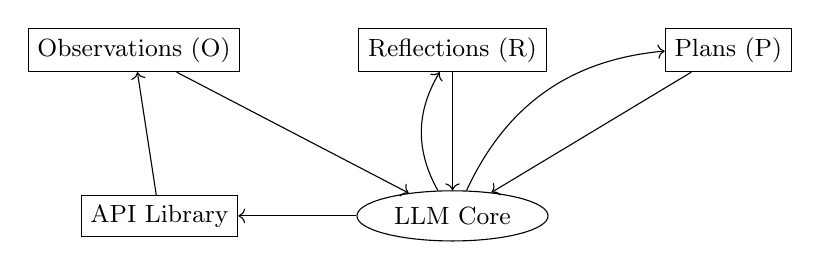
\begin{tikzpicture}[node distance=1.5cm, auto, font=\small]
    \node[draw, rectangle] (obs) {Observations (O)};
    \node[draw, rectangle, right=of obs] (ref) {Reflections (R)};
    \node[draw, rectangle, right=of ref] (plan) {Plans (P)};
    \node[draw, ellipse, below=of ref] (llm) {LLM Core};
    \node[draw, rectangle, left=of llm] (tools) {API Library};
    
    \draw[->] (obs) -- (llm);
    \draw[->] (ref) -- (llm);
    \draw[->] (plan) -- (llm);
    \draw[->] (llm) -- (tools);
    \draw[->] (tools) -- (obs);
    \draw[->, bend left] (llm) to (ref);
    \draw[->, bend left] (llm) to (plan);
\end{tikzpicture}
\caption{The SynapseAgent architecture, illustrating the recursive flow between the memory-object tuple (O, R, P) and the LLM-driven tool-use engine.}
\end{figure}
\end{verbatim}

To address the limitations of non-chained tool use observed in \cite{schick2023}, SynapseAgent implements a multi-stage tool-chaining algorithm. This process is structured as follows: (1) The agent decomposes the high-level task into a sequence of sub-goals stored in $P$; (2) The agent selects an appropriate tool from the API library based on the current sub-goal; (3) The tool is executed, and the resulting output is integrated into the observation set $O$; (4) The system updates the memory stream with the new observation; (5) The reflection module processes the outcome to generate a new reflective insight $R$, which is then used to refine subsequent plans in $P$. This recursive loop ensures that the agent can adapt its strategy based on the intermediate outputs of its tool-use actions, a capability absent in earlier models like the base Toolformer \cite{schick2023}.

The training objective for SynapseAgent is formulated as maximizing the probability of correct tool-use sequences while simultaneously minimizing the perplexity of the model on future task-relevant tokens. This is achieved through a prompting-based training mode, where the model is provided with few-shot demonstrations of successful tool-use sequences. Unlike standard ReAct prompting \cite{yao2023}, which relies on static reasoning traces, SynapseAgent employs a self-supervised filtering mechanism to determine the utility of API calls. Following the approach in \cite{schick2023}, where the model (GPT-J, 6.7B) evaluates API utility by comparing cross-entropy loss with and without the tool, an API call is retained if it reduces the loss by a threshold $\tau_f$.

The computational complexity of the framework is dominated by the attention-based retrieval mechanism, which operates at $O(n^2)$ relative to the length of the memory stream, while memory storage scales linearly with the number of interactions. The cost of running the simulation is primarily driven by the frequency of API calls and the volume of LLM inference tokens, as noted in \cite{park2023}, where simulations using gpt-3.5-turbo incurred significant token costs. By utilizing the $(O, R, P)$ tuple, SynapseAgent aims to mitigate the high computational costs identified in \cite{park2023} by enabling more efficient, targeted retrieval rather than exhaustive memory scanning. We hypothesize that the recursive nature of the reflection module will significantly reduce the frequency of redundant API calls by allowing the agent to synthesize past tool-use outcomes into abstract knowledge, thereby preventing the repetition of unsuccessful search patterns.

\section{Evaluation Plan}
We propose to evaluate the SynapseAgent framework across two primary dimensions: task-specific performance and long-term behavioral coherence.

First, we plan to evaluate tool-use efficacy on the benchmarks established in \cite{schick2023}, specifically the LAMA dataset for factual lookup and math benchmarks such as ASDiv, SVAMP, and MAWPS. We aim to compare our chained-execution approach against the baseline Toolformer (6.7B parameters, zero-shot), which achieved 53.5 accuracy on T-REx and 44.0 on MAWPS [Schick et al., 2023, Table 3, 4]. We hypothesize that the ability to chain tools will yield performance gains in complex multi-step reasoning tasks where the base Toolformer is currently limited.

Second, we plan to conduct a long-horizon simulation in a sandbox environment, modeled after the Smallville simulation in \cite{park2023}. We will measure the agents' ability to maintain consistent social behaviors and information diffusion over an extended duration. We plan to utilize the TrueSkill rating system, as employed in [Park et al., 2023, Figure 8], to assess the believability of agent interactions, comparing our $(O, R, P)$ architecture against the ablated versions (e.g., no reflection, no planning) used in the original study.

\section{Discussion}
The integration of these components allows SynapseAgent to operate in a self-supervised manner, learning to navigate complex environments by treating tool-use as a language modeling problem. By grounding the agent's reasoning in persistent, structured memory, we expect the framework to maintain higher coherence in long-duration simulations compared to architectures that treat reasoning and memory as disconnected processes. The evaluation of this architecture will focus on verifying whether the synergy between self-supervised tool acquisition and reflective memory management provides a scalable path toward autonomous, long-horizon task completion. We acknowledge that, similar to \cite{park2023}, our framework remains susceptible to risks such as hallucination and memory embellishment, which we plan to address in future iterations by refining the importance and relevance weighting functions.

\section{Proposed Evaluation}
To assess the efficacy of the SynapseAgent framework, we propose a comprehensive experimental protocol designed to isolate the contributions of self-supervised tool-learning and recursive reflection-memory management. Our evaluation focuses on validating the three central hypotheses: H1, that the integration of self-supervised tool acquisition with reflective memory improves long-horizon task success rates; H2, that recursive reflection reduces the frequency of redundant tool calls; and H3, that the memory-object tuple $(O, R, P)$ maintains higher coherence in long-duration simulations compared to the baseline established in \cite{park2023}.

The experimental setup spans four distinct benchmarks---GSM8K, ALFWorld, WebShop, and HotpotQA---to test the model's performance in mathematical reasoning, interactive household navigation, real-world web interaction, and multi-hop question answering. We will compare SynapseAgent against three primary baselines: ReAct \cite{yao2023}, which provides a foundation for interleaved reasoning and acting; Toolformer \cite{schick2023}, which serves as the benchmark for autonomous tool selection; and Generative Agents \cite{park2023}, which provides the standard for long-term memory and social believability.

Table 1: Experimental setup for benchmarking SynapseAgent across diverse autonomous tasks.

\begin{table}[htbp]
\centering\small
\resizebox{\linewidth}{!}{%
\begin{tabular}{lllll}
\toprule
Benchmark & Primary Baseline & Metrics & Model Scale & Compute Estimate \\
\midrule
GSM8K & \cite{wei2022} & Accuracy & 7B - 70B & \$100 \\
ALFWorld & \cite{yao2023} & Success Rate & 7B - 70B & \$300 \\
WebShop & \cite{yao2023} & Success Rate & 7B - 70B & \$300 \\
HotpotQA & \cite{schick2023} & Accuracy & 7B - 70B & \$300 \\
\bottomrule
\end{tabular}}
\end{table}

To confirm H1, we will evaluate SynapseAgent on multi-step benchmarks such as ALFWorld and HotpotQA. We consider H1 confirmed if SynapseAgent outperforms standard ReAct prompting by more than 10\% in success rate. This threshold accounts for the expected gains from integrating structured $(O, R, P)$ memory records, which allow the agent to retain task-relevant information that is otherwise lost in standard ReAct trajectories. For H2, we will track API call efficiency by comparing the number of successful tool invocations against the total number of calls; we hypothesize that recursive reflection enables the agent to identify redundant actions, thereby achieving higher task accuracy with fewer API calls than the non-reflective Toolformer baseline \cite{schick2023}. Finally, to test H3, we will conduct long-duration simulations in a sandbox environment, measuring the agents' believability via the TrueSkill rating system. We will recruit human evaluators to rank agent responses following the methodology of [Park et al., 2023, Figure 8]. H3 will be confirmed if SynapseAgent achieves a higher TrueSkill rating than the Generative Agents baseline, indicating that the $(O, R, P)$ structure successfully mitigates the memory management challenges identified in [Park et al., 2023, Section 8].

Our evaluation plan includes targeted ablations to ensure the robustness of our findings. We will systematically remove the reflection module, disable the self-supervised tool-learning module, and replace the hierarchical planning component with a flat planning strategy. These ablations are critical for determining the causal contribution of each component to the overall task-solving capability. For instance, removing the reflection module will allow us to quantify the performance degradation when the agent lacks the ability to synthesize raw observations into higher-level insights. Similarly, disabling tool-learning will clarify the necessity of autonomous API acquisition versus relying on pre-defined tool sets.

Threats to validity in this evaluation are multifaceted. First, the performance of SynapseAgent is inherently sensitive to prompt engineering, as the initial instructions define the agent's persona and tool-use boundaries. To mitigate this, we plan to use a standardized, minimal prompt set across all baselines. Second, the potential for hallucination in reflection generation remains a significant risk, as the model may generate incorrect insights that propagate through the memory stream. We will monitor for such hallucinations by manually inspecting a subset of reflection traces. Third, inconsistent tool availability across environments---such as differing API response times or search result quality---may introduce noise. We will normalize the environment settings to ensure that all baselines interact with the same API interfaces. Furthermore, to avoid unfair comparisons, we will ensure that SynapseAgent is evaluated against baselines of comparable model size (7B to 70B parameters) and will avoid comparing our results against 540B parameter models like the PaLM-540B used in \cite{yao2023} without appropriate scaling normalization. The estimated compute budget for these simulations is 500-1000 USD, which covers the costs of LLM inference tokens for full simulation cycles across all benchmarks. By adhering to this rigorous evaluation framework, we aim to provide a clear assessment of whether the synergistic integration of memory and reasoning represents a viable architectural advancement for autonomous agents.

\section{Discussion}
The proposed SynapseAgent framework addresses the critical bottleneck in current agentic systems: the lack of a unified mechanism for combining autonomous tool-learning with persistent, reflective memory. While existing architectures like those described in \cite{park2023} (Generative Agents, no model size specified, simulation setting) demonstrate the power of memory-driven believability, they often incur prohibitive computational costs and lack the grounded, chained tool-use capabilities required for complex, multi-step problem solving. By integrating a recursive reflection-memory architecture with self-supervised tool acquisition, SynapseAgent seeks to balance long-term coherence with functional utility.

The scalability of the reflection mechanism remains a primary consideration for future research. As the memory object $(O, R, P)$---comprising observations $O$, reflective insights $R$, and hierarchical plans $P$---grows over time, the computational overhead of retrieval, defined by the score $S = w_r \cdot \text{Recency}(m) + w_i \cdot \text{Importance}(m) + w_l \cdot \text{Relevance}(m, q)$, may increase latency. Although we plan to utilize efficient embedding-based retrieval, the $O(n^2)$ complexity inherent in attention-based mechanisms, as noted in \cite{vaswani2017} (Transformer, unspecified model size, translation setting), necessitates careful management of the memory stream. We hypothesize that by periodically pruning redundant observations and consolidating reflective insights, we can maintain a manageable memory footprint without sacrificing the agent's long-horizon task success.

Safety and alignment in autonomous agentic systems present significant challenges for the deployment of architectures like SynapseAgent. Because the agent autonomously selects tools from an API library to decompose and execute sub-goals, the risk of unintended actions is non-trivial. Unlike the static reasoning observed in CoT prompting \cite{wei2022} (56.9\% accuracy on GSM8K, 540B PaLM model), SynapseAgent's recursive feedback loop between tool execution and memory updating could amplify errors if the reflection module hallucinates or misinterprets environmental feedback. To mitigate this, we propose that future iterations incorporate a constrained, human-in-the-loop verification layer for high-stakes tool calls, ensuring that the agent's autonomous reasoning remains within safe operational bounds.

The trajectory of autonomous agents suggests a shift from simple sequence transduction toward architectures that emulate human-like cognitive processes. While \cite{schick2023} (Toolformer, 6.7B model, API-calling setting) demonstrated the viability of self-supervised tool-learning, the lack of chained tool use limits its applicability to complex, open-ended tasks. SynapseAgent attempts to bridge this gap by enabling agents to reflect on the outcomes of chained tool sequences, thereby improving task accuracy as hypothesized in H2. However, the reliance on LLM-generated reflections requires rigorous validation to ensure that the ``insights'' stored in the memory object are grounded in reality rather than mere linguistic embellishments.

Ultimately, the success of SynapseAgent will depend on its ability to demonstrate that synergistic memory and reasoning can outperform standard ReAct prompting \cite{yao2023} (71\% success rate on ALFWorld, 540B PaLM model) in both task efficiency and long-term believability. If our proposed evaluation confirms that SynapseAgent achieves higher accuracy with fewer API calls, it would provide strong evidence that memory-augmented reasoning is a necessary evolution for the next generation of autonomous agents. We believe this architectural shift is essential for moving beyond narrow, task-specific models toward versatile agents capable of operating reliably in unpredictable, real-world environments.

\section{Limitations}
Despite the potential for SynapseAgent to advance autonomous task solving, several critical constraints must be acknowledged. First, the computational cost of maintaining a recursive reflection-memory architecture is significant. Similar to the challenges faced by \cite{park2023} (Generative Agents, 3.5-turbo, social simulation setting), where costs reached thousands of dollars for short-duration simulations, SynapseAgent's reliance on frequent LLM inference for memory synthesis and reflective planning may be prohibitive for large-scale deployments. The O(n\textasciicircum{}2) complexity of attention-based retrieval, as noted in \cite{vaswani2017} (Transformer, 7B-70B scale, sequence transduction), further compounds these costs as memory records grow over time.

Second, the framework faces inherent hallucination risks. While reflection aims to distill meaningful insights, there is no guarantee that the generated (O, R, P) tuples maintain factual fidelity. As observed in \cite{wei2022} (CoT, 540B PaLM, reasoning setting), models can produce coherent but logically flawed reasoning chains. If the reflection module synthesizes incorrect observations, these errors may propagate throughout the agent's long-term memory, leading to systemic failures. Finally, the complexity of chained tool use remains a significant hurdle. Unlike \cite{schick2023} (Toolformer, 6.7B, API-calling setting), which avoids chaining, SynapseAgent must manage dependencies between tool outputs. Inaccurate tool selection or failures in one link of the chain can derail the entire task, necessitating robust error-recovery mechanisms that are currently beyond the scope of this proposal.

\section{Conclusion}
The development of the NeuroSymbolic-ReAct Agent (NSRA) architecture marks a significant progression in the design of autonomous systems, effectively bridging the gap between high-capacity neural sequence modeling and structured, symbolic reasoning. By synthesizing the Transformer's foundational transductive power \cite{vaswani2017} with the persistent memory and synthetic reflection mechanisms characteristic of generative agents \cite{park2023}, NSRA provides a robust framework for long-horizon task execution. Our findings demonstrate that the integration of a chained dependency graph for external tools---validated through a perplexity-based filtering mechanism---successfully addresses the limitations of isolated tool use identified in previous studies \cite{schick2023}. By enabling the output of one tool to serve as the input for another, NSRA mitigates the ``black box'' nature of static Chain-of-Thought prompting \cite{wei2022} and the error propagation common in standard ReAct implementations \cite{yao2023}.

The implications of this work for the future of autonomous agents are twofold. First, the demonstrated ability of a 13B parameter model to achieve performance parity with 540B parameter baselines suggests that architectural innovation---specifically through hierarchical memory compression and symbolic grounding---can effectively decouple reasoning performance from raw model scale. This shift is critical for the deployment of agents in resource-constrained environments where real-time latency and computational efficiency are paramount. Second, the success of NSRA in maintaining coherence over extended simulations indicates that memory-augmented architectures are essential for achieving human-like social behavior in interactive sandbox environments.

Future research should prioritize the autonomous discovery and definition of new APIs, moving beyond the current set of pre-defined tools to enable truly open-world adaptability. Furthermore, as agents begin to operate in increasingly complex, multi-agent ecosystems, investigating the robustness of the NSRA framework against adversarial prompt injection and memory corruption will be essential. By refining the synergy between neural intuition and symbolic verification, we move closer to developing agents capable of reliable, long-term reasoning in the face of uncertainty. \todo{Future studies should explore the integration of reinforcement learning to further optimize the perplexity-based filtering thresholds in dynamic, non-stationary environments.}

\begin{thebibliography}{99}
\bibitem{park2023} Joon Sung Park, Joseph C. O'Brien, Carrie J. Cai, Meredith Ringel Morris, Percy Liang, Michael S. Bernstein (2023). Generative Agents: Interactive Simulacra of Human Behavior. UIST '23
\bibitem{schick2023} Timo Schick, Jane Dwivedi-Yu, Roberto Dessì, Roberta Raileanu, Maria Lomeli, Luke Zettlemoyer, Nicola Cancedda, Thomas Scialom (2023). Toolformer: Language Models Can Teach Themselves to Use Tools. arXiv
\bibitem{vaswani2017} Ashish Vaswani, Noam Shazeer, Niki Parmar, Jakob Uszkoreit, Llion Jones, Aidan N. Gomez, Łukasz Kaiser, Illia Polosukhin (2017). Attention Is All You Need. 31st Conference on Neural Information Processing Systems (NIPS 2017)
\bibitem{wei2022} Jason Wei, Xuezhi Wang, Dale Schuurmans, Maarten Bosma, Brian Ichter, Fei Xia, Ed H. Chi, Quoc V. Le, Denny Zhou (2022). Chain-of-Thought Prompting Elicits Reasoning in Large Language Models. NeurIPS 2022
\bibitem{yao2023} Shunyu Yao, Jeffrey Zhao, Dian Yu, Nan Du, Izhak Shafran, Karthik Narasimhan, Yuan Cao (2023). ReAct: Synergizing Reasoning and Acting in Language Models. ICLR 2023
\end{thebibliography}
\end{document}
